\documentclass[12pt,a4paper]{article}
\usepackage[utf8]{inputenc}
\usepackage{tikz}
\usetikzlibrary{shapes,arrows,positioning,decorations.pathreplacing,calc,fit,backgrounds}
\usepackage{geometry}
\geometry{margin=1in}

\title{Legacy HR Portal System Architecture Diagram}
\author{System Documentation}
\date{\today}

\begin{document}

\maketitle

\section{System Overview}

This document provides a system architecture view of the Legacy HR Portal, a single-host internal HR application built with PHP, Apache, and MySQL. It highlights core components, data flow, trust boundaries, and known risk areas used for threat modeling.

\section{High-Level System Architecture}
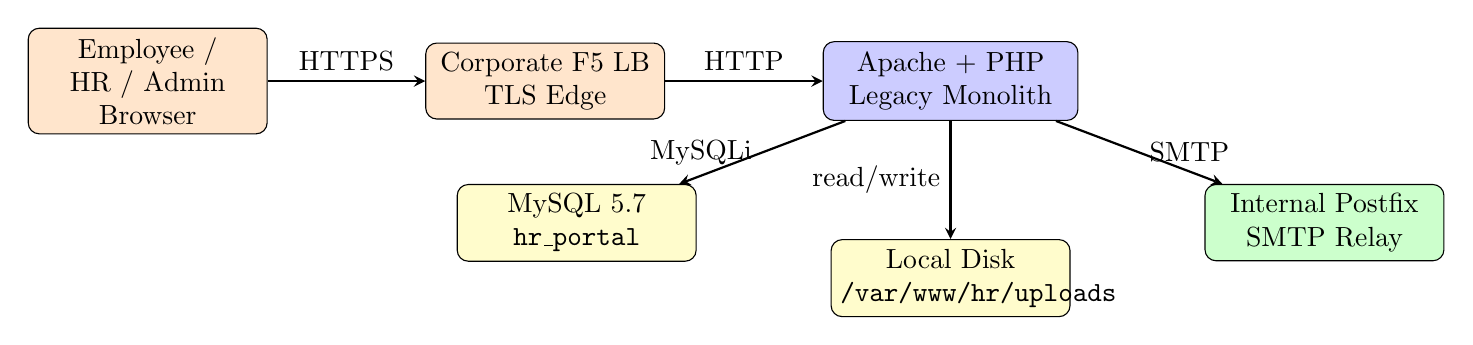
\begin{tikzpicture}[
    node distance=1.5cm and 2cm,
    box/.style={rectangle, draw, fill=blue!20, text width=3cm, text centered, minimum height=1cm, rounded corners},
    service/.style={rectangle, draw, fill=green!20, text width=2.8cm, text centered, minimum height=0.9cm, rounded corners},
    external/.style={rectangle, draw, fill=orange!20, text width=2.8cm, text centered, minimum height=0.9cm, rounded corners},
    data/.style={rectangle, draw, fill=yellow!20, text width=2.8cm, text centered, minimum height=0.9cm, rounded corners},
    arrow/.style={->, >=stealth, thick}
]
    \node[external] (users) {Employee / HR / Admin\\Browser};
    \node[external, right=of users] (f5) {Corporate F5 LB\\TLS Edge};
    \node[box, right=of f5] (apache) {Apache + PHP\\Legacy Monolith};
    \node[data, below=of apache] (disk) {Local Disk\\\texttt{/var/www/hr/uploads}};
    \node[data, below left=0.8cm and 1.6cm of apache] (mysql) {MySQL 5.7\\\texttt{hr\_portal}};
    \node[service, below right=0.8cm and 1.6cm of apache] (smtp) {Internal Postfix\\SMTP Relay};

    \draw[arrow] (users) -- node[above] {HTTPS} (f5);
    \draw[arrow] (f5) -- node[above] {HTTP} (apache);
    \draw[arrow] (apache) -- node[left] {read/write} (disk);
    \draw[arrow] (apache) -- node[left] {MySQLi} (mysql);
    \draw[arrow] (apache) -- node[right] {SMTP} (smtp);
\end{tikzpicture}

\newpage

\section{Application Components}
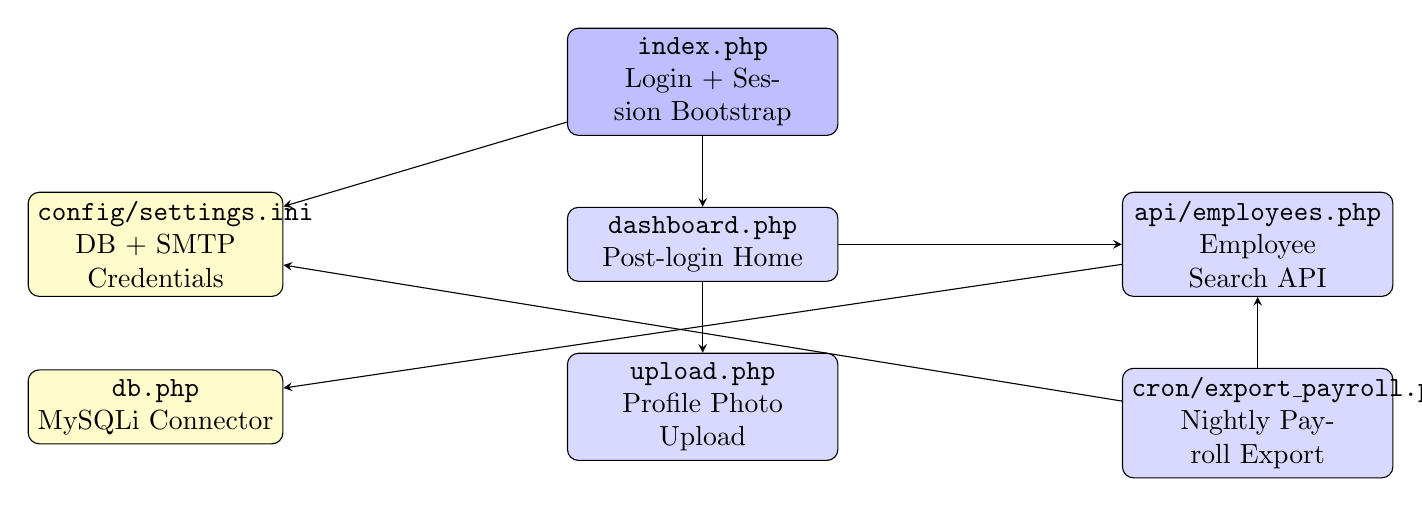
\begin{tikzpicture}[
    node distance=0.9cm and 1.6cm,
    component/.style={rectangle, draw, fill=blue!15, text width=3.2cm, text centered, minimum height=0.8cm, rounded corners},
    data/.style={rectangle, draw, fill=yellow!20, text width=3.0cm, text centered, minimum height=0.8cm, rounded corners},
    arrow/.style={->, >=stealth}
]
    \node[component, fill=blue!25] (index) {\texttt{index.php}\\Login + Session Bootstrap};
    \node[component, below=of index] (dashboard) {\texttt{dashboard.php}\\Post-login Home};
    \node[component, below=of dashboard] (upload) {\texttt{upload.php}\\Profile Photo Upload};
    \node[component, right=3.6cm of dashboard] (api) {\texttt{api/employees.php}\\Employee Search API};
    \node[component, below=of api] (cron) {\texttt{cron/export\_payroll.php}\\Nightly Payroll Export};

    \node[data, left=3.6cm of dashboard] (cfg) {\texttt{config/settings.ini}\\DB + SMTP Credentials};
    \node[data, left=3.6cm of upload] (dbhelper) {\texttt{db.php}\\MySQLi Connector};

    \draw[arrow] (index) -- (dashboard);
    \draw[arrow] (dashboard) -- (upload);
    \draw[arrow] (dashboard) -- (api);
    \draw[arrow] (cron) -- (api);
    \draw[arrow] (index) -- (cfg);
    \draw[arrow] (api) -- (dbhelper);
    \draw[arrow] (cron) -- (cfg);
\end{tikzpicture}

\newpage

\section{Trust Boundaries and Data Stores}
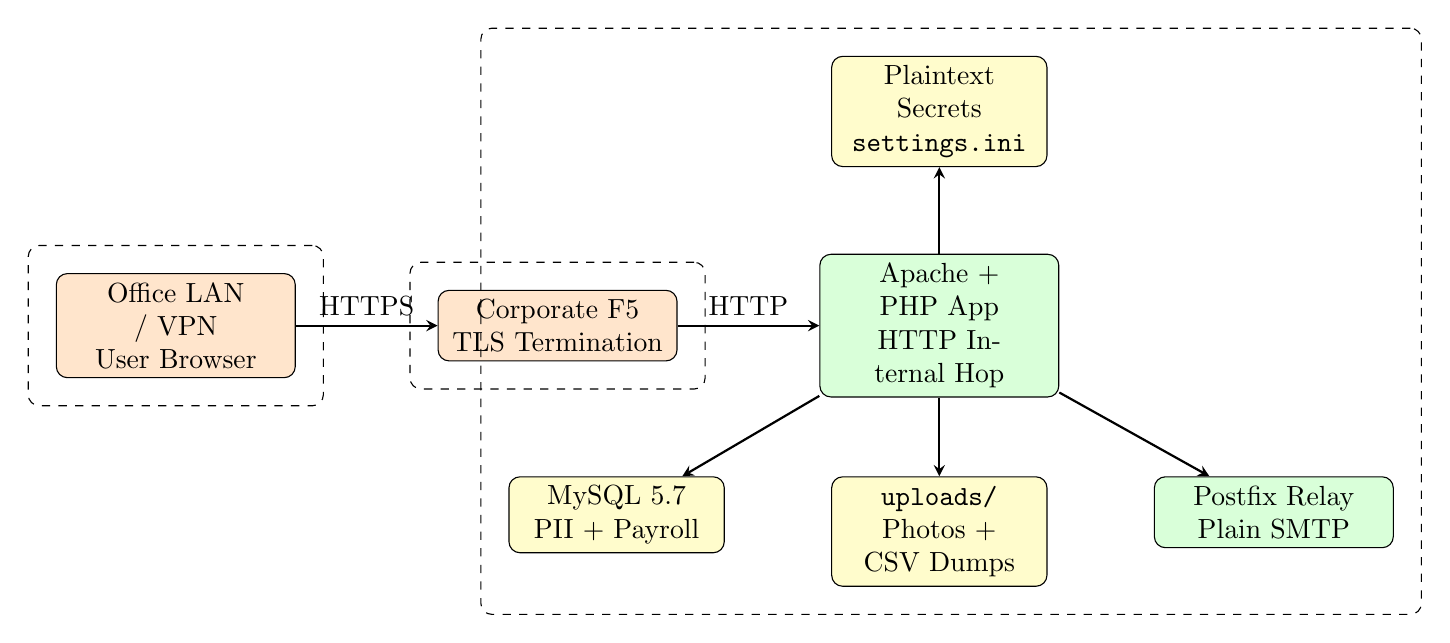
\begin{tikzpicture}[
    node distance=1.1cm and 1.8cm,
    zone/.style={rectangle, draw, dashed, rounded corners, inner sep=0.35cm},
    nodebox/.style={rectangle, draw, fill=green!15, text width=2.8cm, text centered, minimum height=0.8cm, rounded corners},
    data/.style={rectangle, draw, fill=yellow!20, text width=2.5cm, text centered, minimum height=0.75cm, rounded corners},
    external/.style={rectangle, draw, fill=orange!20, text width=2.8cm, text centered, minimum height=0.8cm, rounded corners},
    arrow/.style={->, >=stealth, thick}
]
    \node[external] (browser) {Office LAN / VPN\\User Browser};
    \node[external, right=of browser] (lb) {Corporate F5\\TLS Termination};
    \node[nodebox, right=of lb] (app) {Apache + PHP App\\HTTP Internal Hop};
    \node[data, above=of app] (ini) {Plaintext Secrets\\\texttt{settings.ini}};
    \node[data, below left=1cm and 1.2cm of app] (db) {MySQL 5.7\\PII + Payroll};
    \node[data, below=1cm of app] (uploads) {\texttt{uploads/}\\Photos + CSV Dumps};
    \node[nodebox, below right=1cm and 1.2cm of app] (relay) {Postfix Relay\\Plain SMTP};

    \node[zone, fit=(browser)] {};
    \node[zone, fit=(lb)] {};
    \node[zone, fit=(app)(ini)(db)(uploads)(relay)] {};

    \draw[arrow] (browser) -- node[above] {HTTPS} (lb);
    \draw[arrow] (lb) -- node[above] {HTTP} (app);
    \draw[arrow] (app) -- (ini);
    \draw[arrow] (app) -- (db);
    \draw[arrow] (app) -- (uploads);
    \draw[arrow] (app) -- (relay);
\end{tikzpicture}

\newpage

\section{Payroll Export Pipeline}
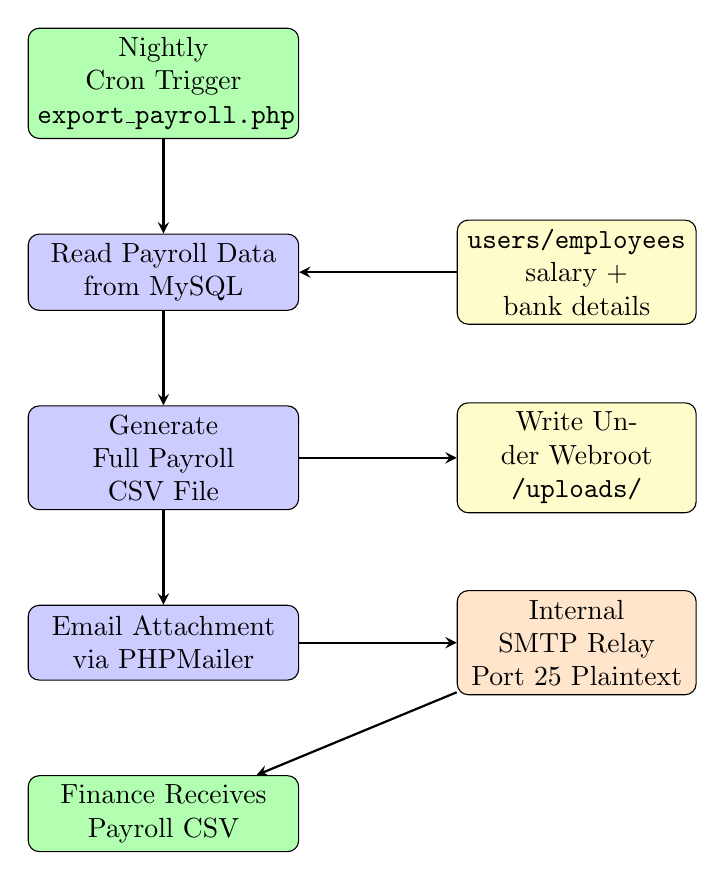
\begin{tikzpicture}[
    node distance=1.2cm and 2cm,
    process/.style={rectangle, draw, fill=blue!20, text width=3.2cm, text centered, minimum height=0.95cm, rounded corners},
    data/.style={rectangle, draw, fill=yellow!20, text width=2.8cm, text centered, minimum height=0.8cm, rounded corners},
    external/.style={rectangle, draw, fill=orange!20, text width=2.8cm, text centered, minimum height=0.8cm, rounded corners},
    arrow/.style={->, >=stealth, thick}
]
    \node[process, fill=green!30] (trigger) {Nightly Cron Trigger\\\texttt{export\_payroll.php}};
    \node[process, below=of trigger] (query) {Read Payroll Data\\from MySQL};
    \node[data, right=of query] (db) {\texttt{users/employees}\\salary + bank details};
    \node[process, below=of query] (csv) {Generate Full Payroll\\CSV File};
    \node[data, right=of csv] (webroot) {Write Under Webroot\\\texttt{/uploads/}};
    \node[process, below=of csv] (mail) {Email Attachment\\via PHPMailer};
    \node[external, right=of mail] (smtp) {Internal SMTP Relay\\Port 25 Plaintext};
    \node[process, below=of mail, fill=green!30] (finance) {Finance Receives\\Payroll CSV};

    \draw[arrow] (trigger) -- (query);
    \draw[arrow] (db) -- (query);
    \draw[arrow] (query) -- (csv);
    \draw[arrow] (csv) -- (webroot);
    \draw[arrow] (csv) -- (mail);
    \draw[arrow] (mail) -- (smtp);
    \draw[arrow] (smtp) -- (finance);
\end{tikzpicture}

\newpage

\section{Authentication and Access Flow}
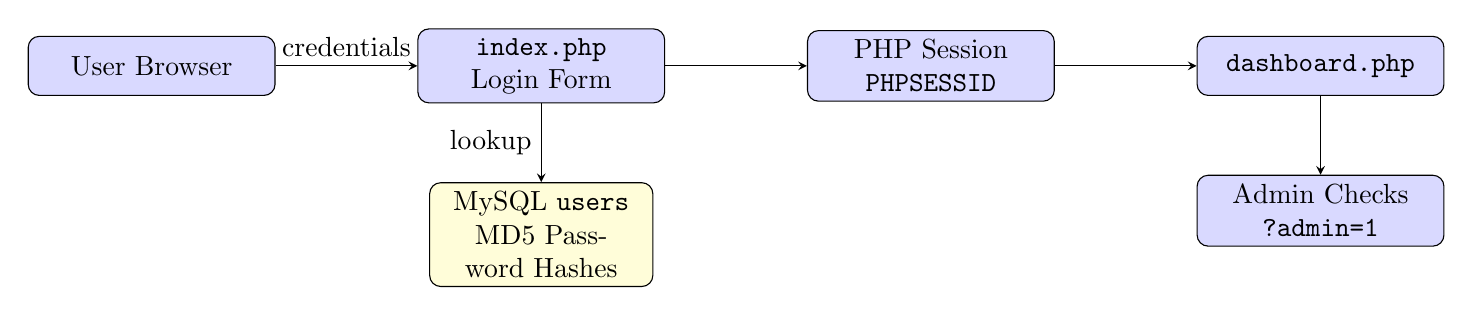
\begin{tikzpicture}[
    node distance=1.0cm and 1.8cm,
    component/.style={rectangle, draw, fill=blue!15, text width=2.9cm, text centered, minimum height=0.75cm, rounded corners},
    data/.style={rectangle, draw, fill=yellow!15, text width=2.6cm, text centered, minimum height=0.7cm, rounded corners},
    arrow/.style={->, >=stealth}
]
    \node[component] (user) {User Browser};
    \node[component, right=of user] (login) {\texttt{index.php}\\Login Form};
    \node[data, below=of login] (users) {MySQL \texttt{users}\\MD5 Password Hashes};
    \node[component, right=of login] (session) {PHP Session\\\texttt{PHPSESSID}};
    \node[component, right=of session] (dash) {\texttt{dashboard.php}};
    \node[component, below=of dash] (admin) {Admin Checks\\\texttt{?admin=1}};

    \draw[arrow] (user) -- node[above] {credentials} (login);
    \draw[arrow] (login) -- node[left] {lookup} (users);
    \draw[arrow] (login) -- (session);
    \draw[arrow] (session) -- (dash);
    \draw[arrow] (dash) -- (admin);
\end{tikzpicture}

\newpage

\section{Primary Attack Surface}
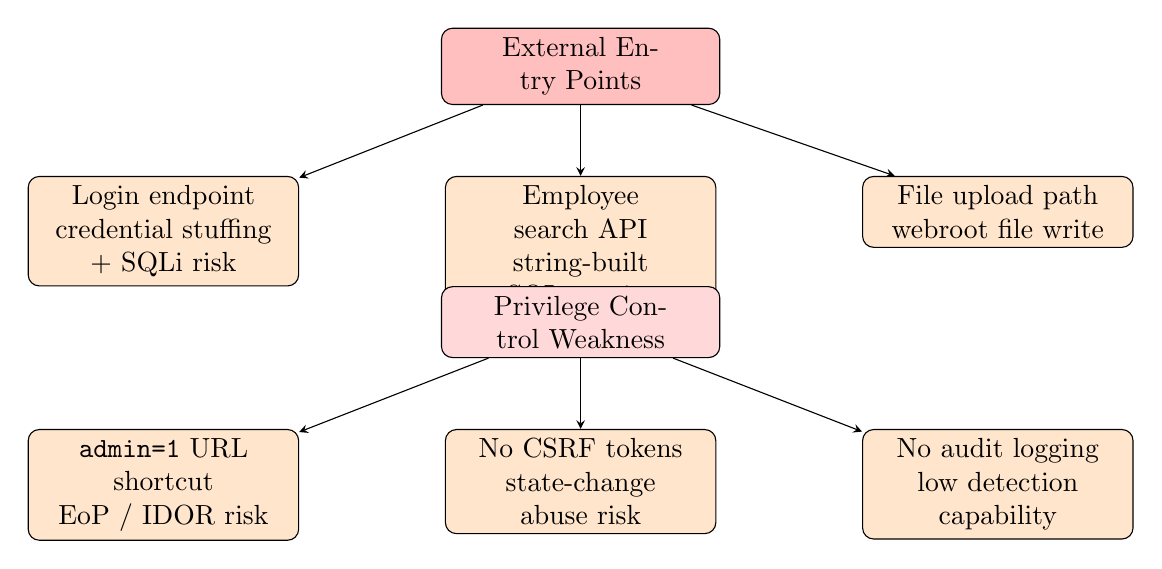
\begin{tikzpicture}[
    node distance=0.9cm and 1.8cm,
    surface/.style={rectangle, draw, fill=red!15, text width=3.3cm, text centered, minimum height=0.8cm, rounded corners},
    detail/.style={rectangle, draw, fill=orange!20, text width=3.2cm, text centered, minimum height=0.75cm, rounded corners},
    arrow/.style={->, >=stealth}
]
    \node[surface, fill=red!25] (entry) {External Entry Points};
    \node[detail, below left=of entry] (login) {Login endpoint\\credential stuffing + SQLi risk};
    \node[detail, below=of entry] (search) {Employee search API\\string-built SQL queries};
    \node[detail, below right=of entry] (upload) {File upload path\\webroot file write};
    \node[surface, below=2.3cm of entry] (priv) {Privilege Control Weakness};
    \node[detail, below left=of priv] (admin) {\texttt{admin=1} URL shortcut\\EoP / IDOR risk};
    \node[detail, below=of priv] (csrf) {No CSRF tokens\\state-change abuse risk};
    \node[detail, below right=of priv] (audit) {No audit logging\\low detection capability};

    \draw[arrow] (entry) -- (login);
    \draw[arrow] (entry) -- (search);
    \draw[arrow] (entry) -- (upload);
    \draw[arrow] (priv) -- (admin);
    \draw[arrow] (priv) -- (csrf);
    \draw[arrow] (priv) -- (audit);
\end{tikzpicture}

\newpage

\section{Data Classification and Handling}
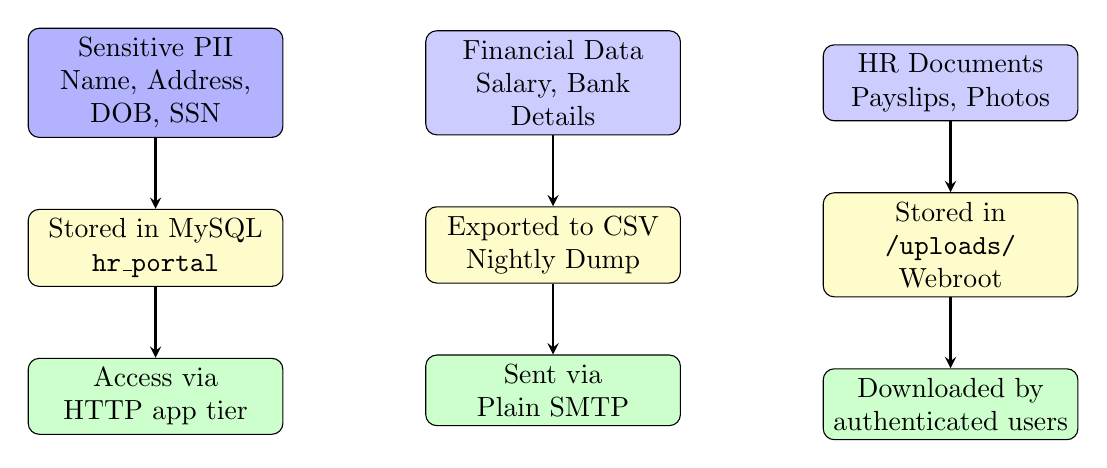
\begin{tikzpicture}[
    node distance=0.9cm and 1.8cm,
    class/.style={rectangle, draw, fill=blue!20, text width=3.0cm, text centered, minimum height=0.8cm, rounded corners},
    store/.style={rectangle, draw, fill=yellow!20, text width=3.0cm, text centered, minimum height=0.8cm, rounded corners},
    flow/.style={rectangle, draw, fill=green!20, text width=3.0cm, text centered, minimum height=0.8cm, rounded corners},
    arrow/.style={->, >=stealth, thick}
]
    \node[class, fill=blue!30] (pii) {Sensitive PII\\Name, Address, DOB, SSN};
    \node[class, right=of pii] (finance) {Financial Data\\Salary, Bank Details};
    \node[class, right=of finance] (docs) {HR Documents\\Payslips, Photos};

    \node[store, below=of pii] (db) {Stored in MySQL\\\texttt{hr\_portal}};
    \node[store, below=of finance] (csv) {Exported to CSV\\Nightly Dump};
    \node[store, below=of docs] (uploads) {Stored in\\\texttt{/uploads/} Webroot};

    \node[flow, below=of db] (web) {Access via\\HTTP app tier};
    \node[flow, below=of csv] (mail) {Sent via\\Plain SMTP};
    \node[flow, below=of uploads] (download) {Downloaded by\\authenticated users};

    \draw[arrow] (pii) -- (db);
    \draw[arrow] (finance) -- (csv);
    \draw[arrow] (docs) -- (uploads);
    \draw[arrow] (db) -- (web);
    \draw[arrow] (csv) -- (mail);
    \draw[arrow] (uploads) -- (download);
\end{tikzpicture}

\newpage

\section{Legacy Technology Dependencies}
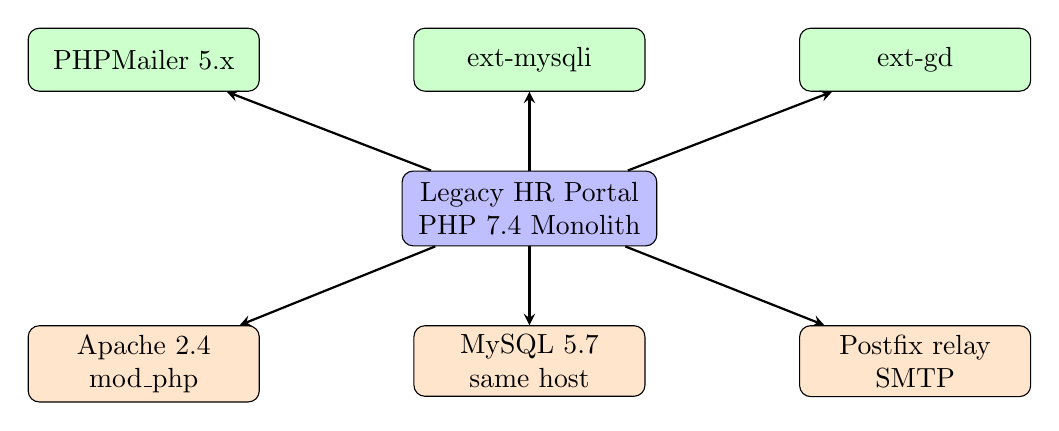
\begin{tikzpicture}[
    node distance=1cm and 1.8cm,
    core/.style={rectangle, draw, fill=blue!25, text width=3cm, text centered, minimum height=0.95cm, rounded corners},
    dep/.style={rectangle, draw, fill=green!20, text width=2.7cm, text centered, minimum height=0.8cm, rounded corners},
    infra/.style={rectangle, draw, fill=orange!20, text width=2.7cm, text centered, minimum height=0.8cm, rounded corners},
    arrow/.style={->, >=stealth, thick}
]
    \node[core] (app) {Legacy HR Portal\\PHP 7.4 Monolith};
    \node[dep, above left=of app] (phpmailer) {PHPMailer 5.x};
    \node[dep, above=of app] (mysqli) {ext-mysqli};
    \node[dep, above right=of app] (gd) {ext-gd};
    \node[infra, below left=of app] (apache) {Apache 2.4\\mod\_php};
    \node[infra, below=of app] (mysql) {MySQL 5.7\\same host};
    \node[infra, below right=of app] (postfix) {Postfix relay\\SMTP};

    \draw[arrow] (app) -- (phpmailer);
    \draw[arrow] (app) -- (mysqli);
    \draw[arrow] (app) -- (gd);
    \draw[arrow] (app) -- (apache);
    \draw[arrow] (app) -- (mysql);
    \draw[arrow] (app) -- (postfix);
\end{tikzpicture}

\newpage

\section{Complete Legacy System Integration}
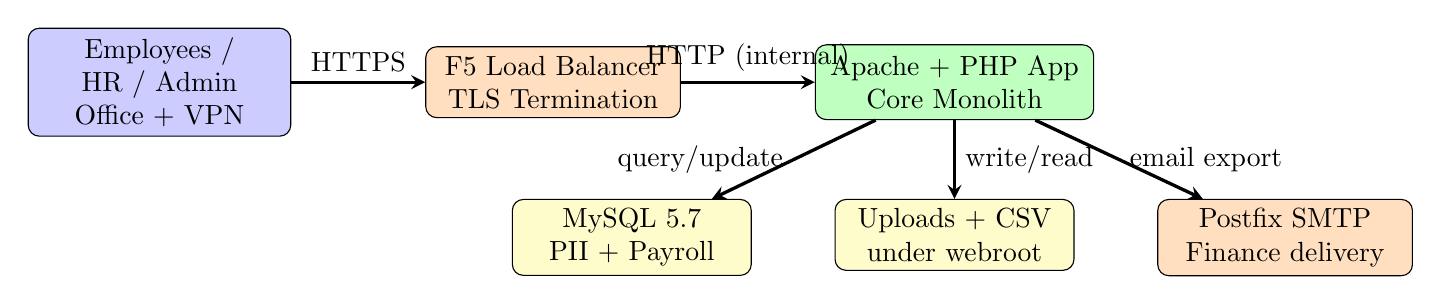
\begin{tikzpicture}[
    node distance=1cm and 1.7cm,
    user/.style={rectangle, draw, fill=blue!20, text width=3.1cm, text centered, minimum height=0.9cm, rounded corners},
    app/.style={rectangle, draw, fill=green!25, text width=3.3cm, text centered, minimum height=0.95cm, rounded corners},
    ext/.style={rectangle, draw, fill=orange!25, text width=3.0cm, text centered, minimum height=0.85cm, rounded corners},
    data/.style={rectangle, draw, fill=yellow!20, text width=2.8cm, text centered, minimum height=0.8cm, rounded corners},
    arrow/.style={->, >=stealth, very thick}
]
    \node[user] (browser) {Employees / HR / Admin\\Office + VPN};
    \node[ext, right=of browser] (lb) {F5 Load Balancer\\TLS Termination};
    \node[app, right=of lb] (php) {Apache + PHP App\\Core Monolith};
    \node[data, below left=1cm and 0.8cm of php] (mysql) {MySQL 5.7\\PII + Payroll};
    \node[data, below=1cm of php] (files) {Uploads + CSV\\under webroot};
    \node[ext, below right=1cm and 0.8cm of php] (relay) {Postfix SMTP\\Finance delivery};

    \draw[arrow] (browser) -- node[above] {HTTPS} (lb);
    \draw[arrow] (lb) -- node[above] {HTTP (internal)} (php);
    \draw[arrow] (php) -- node[left] {query/update} (mysql);
    \draw[arrow] (php) -- node[right] {write/read} (files);
    \draw[arrow] (php) -- node[right] {email export} (relay);
\end{tikzpicture}

\section{Summary}

This architecture documentation covers:
\begin{itemize}
    \item \textbf{System Topology}: Browser, load balancer, monolith, data stores, and mail relay.
    \item \textbf{Component Breakdown}: Major PHP entry points and scheduled workflows.
    \item \textbf{Trust Boundaries}: TLS termination, internal plaintext links, and local storage boundaries.
    \item \textbf{Payroll Workflow}: Nightly export path from database to CSV email attachment.
    \item \textbf{Auth Path}: Session establishment and privileged route behavior.
    \item \textbf{Attack Surface}: Injection, privilege escalation, upload abuse, and monitoring gaps.
    \item \textbf{Sensitive Data Handling}: Storage and transfer paths for PII and financial records.
    \item \textbf{Dependency Model}: Legacy runtime libraries and infrastructure components.
\end{itemize}

The Legacy HR Portal uses a classic monolithic architecture with co-located services and limited security controls. This structure makes it a useful reference system for threat modeling, especially for STRIDE analyses focused on spoofing, tampering, information disclosure, and elevation of privilege.

\end{document}
